%!TEX root = ../var.tex

Пусть $(\Omega,\mathfrak{A},\P)$-- произвольное вероятностное пространство.

\begin{definition}
\label{def:15.1}
	Вектор $(\xi_1, \dots, \xi_n)$ называется случайным вектором, если $\xi_1, \dots, \xi_n$ являются случайными величинами, заданными на одном
и том же вероятностном пространстве $\Omega$.
\end{definition}

\begin{definition}
\label{def:15.2}
	Функцией совместного распределения случайных
величин $(\xi_1, \dots, \xi_n)$ (или случайного вектора $(\xi_1, \dots, \xi_n)$) называется функция $F_{\xi_1, \dots, \xi_n} : \mathbb{R}^n \rightarrow [0, 1]$, определённая по формуле
\begin{equation*}
	F_{\xi_1, \dots, \xi_n}(x_1,\dots,x_n)=\P(\xi_1\leqslant x_1,\dots,\xi_n\leqslant x_n).
\end{equation*}

Ясно, что $0 \leqslant F_{\xi_1, \dots, \xi_n}(x_1,\dots,x_n) \leqslant 1$

\end{definition}

\begin{definition}
\label{def:15.3}
	Говорят, что случайные величины $(\xi_1, \dots, \xi_n)$ имеют абсолютно непрерывное совместное распределение, если существует
такая неотрицательная функция $f_{\xi_1, \dots, \xi_n}(x_1,\dots,x_n)$, что для любой точки
$(x_1,\dots,x_n)\in\mathbb{R}^n$ функция распределения $F_{\xi_1, \dots, \xi_n}(x_1,\dots,x_n)$ представима в
виде
\begin{equation*}
	F_{\xi_1, \dots, \xi_n}(x_1,\dots,x_n)=\int\limits_{-\infty}^{x_1}\ldots
	\int\limits_{-\infty}^{x_n}f_{\xi_1, \dots, \xi_n}(t_1,\dots,t_n)dt_1\ldots dt_n.
\end{equation*}
При этом функция $f_{\xi_1, \dots, \xi_n}(x_1,\dots,x_n)$ называется плотностью вероятности совместного распределения случайных величин ${\xi_1, \dots, \xi_n}$.
\end{definition}

\begin{lemma}
\label{lemma:15.4}
Справедлива формула
	\begin{equation*}
		f_{\xi_1, \dots, \xi_n}(x_1,\dots,x_n)=\frac
		{\partial^nF_{\xi_1, \dots, \xi_n}(x_1,\dots,x_n)}
		{\partial x_1\ldots \partial x_n}.
	\end{equation*}
\end{lemma}

\begin{proof}
	Формула получается в результате последовательного дифференцирования формулы определения \ref{def:15.3} по верхним пределам.
\end{proof}

\begin{definition}
\label{def:15.5}
	Случайные величины $\xi_1, \dots, \xi_n$ называются независимыми, если для любого набора множеств $A_1,\dots ,A_n \subset \mathbb{R}$, такого что\newline
 	$\xi_1^{-1}(A_1), \dots, \xi_n^{-1}(A_n)\in\mathfrak{A}$ иммет место равенство
 	\begin{equation*}
 		\P(\xi_1\in A_1,\dots,\xi_n\in A_n)=\P(\xi_1 \in A_1)\cdot\ldots\cdot\P(\xi_m\in A_n).
 	\end{equation*}
\end{definition}

 \begin{lemma}\-
\label{lemma:15.6}

 \begin{enumerate}
 	\item Случайные величины независимы, если для любых $$x_1,\dots, x_n \in \mathbb{R}$$ имеет место равенство
 	\begin{equation*}
 		F_{\xi_1, \dots, \xi_n}(x_1,\dots,x_n)=F_{\xi_1}(x_1)\cdot\ldots\cdot F_{\xi_n}(x_n).
 	\end{equation*}
 	\item Случайные величины независимы, если для любых $x_1,\ldots,x_n\in\mathbb{R}$ имеет место равенство
 	\begin{equation*}
		f_{\xi_1, \dots, \xi_n}(x_1,\dots,x_n)=f_{\xi_1}(x_1)\cdot\ldots\cdot f_{\xi_n}(x_n). 		
 	\end{equation*}
 \end{enumerate}
\end{lemma}

\begin{proof}\-

	1)
	\begin{gather*}
	F_{\xi_1, \dots, \xi_n}(x_1,\dots,x_n)=\P(\xi_1\leqslant x_1,\ldots,\xi_n
	\leqslant x_n)=\\=
	\P(\xi_1\leqslant x_1)\cdot\ldots\cdot\P(\xi_n\leqslant x_n)=F_{\xi_1}(x_1)\cdot\ldots\cdot F_{\xi_n}(x_n).
	\end{gather*}	

	2)
	\begin{gather*}
	f_{\xi_1,\ldots,\xi_n}(x_1,\ldots,x_n)=
		\frac
		{\partial^nF_{\xi_1, \dots, \xi_n}(x_1,\dots,x_n)}
		{\partial x_1\ldots \partial x_n}=
		\frac
		{\partial^n\left[F_{\xi_1}(x_1)\cdot\ldots\cdot F_{\xi_n}(x_n)\right]}
		{\partial x_1\ldots \partial x_n}=\\=
		\frac{\partial F_{\xi_1}(x_1)}{\partial x_1}\cdot\ldots\cdot
		\frac{\partial F_{\xi_n}(x_n)}{\partial x_n}=f_{\xi_1}(x_1)\cdot\ldots\cdot f_{\xi_n}(x_n).
	\end{gather*}
\end{proof}

В следующей теореме без потери общности и для простоты формулировки мы ограничимся двухмерным случаем, $n = 2$.

\begin{theorem}[Свойства функции распределения, без доказательства]
\label{th:15.7}
.
\begin{enumerate}
	\item Функция $F_{\xi_1,\xi_2}(x_1,x_2)$ является неубывающей по каждому аргументу $x_1$ и $x_2$.

	\item Существуют пределы 
	\begin{gather*}
	F_{\xi_1,\xi_2}(-\infty,x_2)=\lim\limits_{x_1\to-\infty}
	F_{\xi_1,\xi_2}(x_1,x_2)=0 \\
	F_{\xi_1,\xi_2}(x_1,-\infty)=\lim\limits_{x_2\to-\infty}
	F_{\xi_1,\xi_2}(x_1,x_2)=0
	\end{gather*}

	\item Существуют пределы 
	\begin{gather*}
	F_{\xi_1,\xi_2}(\infty,x_2)=\lim\limits_{x_1\to\infty}
	F_{\xi_1,\xi_2}(x_1,x_2)=F_{\xi_2}(x_2) \\
	F_{\xi_1,\xi_2}(x_1,\infty)=\lim\limits_{x_2\to\infty}
	F_{\xi_1,\xi_2}(x_1,x_2)=F_{\xi_1}(x_1)
	\end{gather*}

	\item Справедливо
	\begin{gather*}
	f_{\xi_1}(x_1)=\int\limits_{-\infty}^{\infty}f_{\xi_1,\xi_2}(x_1,x_2)dx_2, \\
	f_{\xi_2}(x_2)=\int\limits_{-\infty}^{\infty}f_{\xi_1,\xi_2}(x_1,x_2)dx_1,
	\end{gather*}

	\item $F_{\xi,\eta}(x, y)$ непрерывна справа по каждой координате x и y.



\end{enumerate}

\end{theorem}

\begin{example}\-
\label{ex:15.8}
	\begin{enumerate}
		\item Пусть $A \subset \mathbb{R}_n$ — множество, имеющее конечный
			объём $\mu(A)$, в пространстве с координатами $x = (x_1,\dots, x_n)$. Тогда функция
			\begin{equation*}
				f_{\xi_1,\dots,\xi_n}(x_1,\dots,x+n)=
				\begin{cases}
					\frac{1}{\mu(A)}, &\text{ если } x\in A\\
					0, &\text{ если } x\notin A\\
				\end{cases}
			\end{equation*}
			определяет плотность случайного вектора $\{\xi_1,\dots,\xi_n\}$ с равномерным распределением в $A$.
	\end{enumerate}
		\item Функция $f_{\xi,\eta}(x,y)=$
		\begin{equation*}
			=\frac{1}{2\pi\sigma_1\sigma_2\sqrt{1-r^2}}\exp
			\left\{
				-\frac{1}{2(1-r^2)}
			\left[
				\frac{(x-a)^2}{\sigma_1^2}-\frac{2r(x-a)(y-b)}{\sigma_1\sigma_2}+\frac{(y-b)^2}{\sigma_2^2} 
			\right] 
			\right\},
		\end{equation*}
		где $r$ — коэффициент корреляции (см. \S\ref{par:18}), определяет двухмерную нормальную плотность вероятности случайного вектора $(\xi, \eta)$, показанную на рис. \ref{fig21}. Там же показан эллипс равных вероятностей
		\begin{equation*}
			\frac{(x-a)^2}{\sigma_1^2}-\frac{2r(x-a)(y-b)}{\sigma_1\sigma_2}+\frac{(y-b)^2}{\sigma_2^2}=const
		\end{equation*}
\begin{figure}[H]
	\centering
	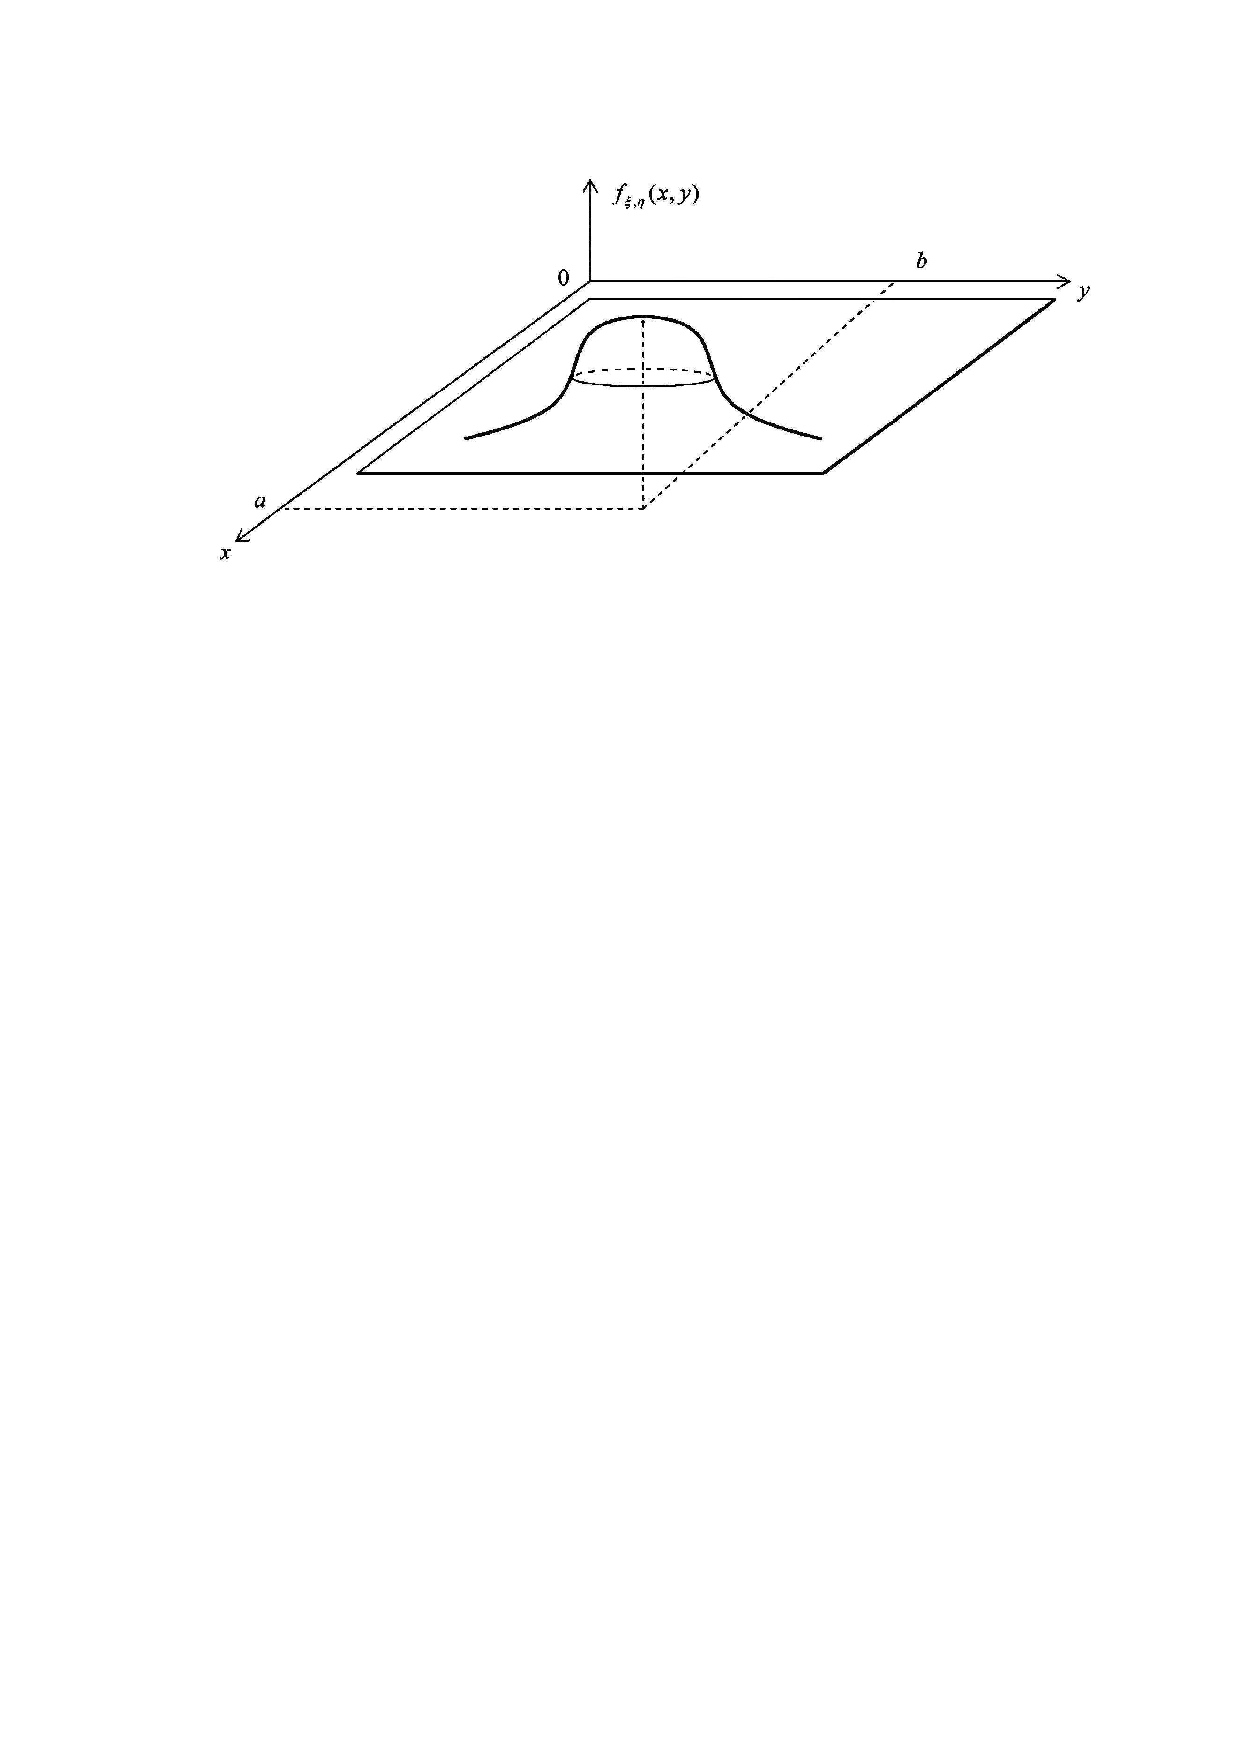
\includegraphics[]{pic/pic21}
	\caption{Плотность вероятности двухмерного нормального распределения.}
	\label{fig21}
\end{figure}
\end{example}
